% !TEX root = ../presentation.tex
% Convnets

\begin{slide}{Convolutional Layers}
  \only<2>{
    \includegraphics[scale=0.25]{burger}
  }
  \only<3>{
    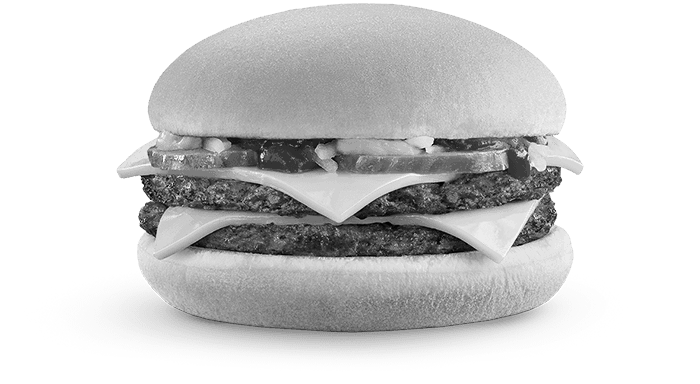
\includegraphics[scale=0.25]{burger-bw}
  }
\end{slide}

\begin{slide}{Convolutional Layers}
  \begin{tikzpicture}
    % Image
    \draw (0, 0) grid ++(3, 3);

    % Grayscale pixel values
    \only<1>{
      \foreach \x in {0, ..., 2} {
        \foreach \y in {0, ..., 2} {
          \randomgray
          \fill [randomgray] (\x, \y) rectangle ++(1, 1);
        }
      }
    }

    \only<2-3>{
      \draw (0.5, 0.5) node {$0.8$};
      \draw (1.5, 0.5) node {$0.3$};
      \draw (2.5, 0.5) node {$0.5$};
      \draw (0.5, 1.5) node {$0.7$};
      \draw (1.5, 1.5) node {$0.2$};
      \draw (2.5, 1.5) node {$0.6$};
      \draw (0.5, 2.5) node {$0.4$};
      \draw (1.5, 2.5) node {$0.9$};
      \draw (2.5, 2.5) node {$0.1$};
    }

    \draw (1.5, -0.5) node {Image};

    \only<3>{
      \draw (4, 0) grid ++(2, 2);

      \draw (4.5, 0.5) node {$3.1$};
      \draw (5.5, 0.5) node {$0.9$};
      \draw (4.5, 1.5) node {$5.7$};
      \draw (5.5, 1.5) node {$2.4$};

      \draw (5, -0.5) node {Kernel};
    }

    \only<4-5>{
      \draw (0.5, 0.5) node {$0.8$};
      \draw (1.5, 0.5) node {$0.3$};
      \draw (2.5, 0.5) node {$0.5$};
      \draw (0.5, 1.5) node {\tiny$3.1 \cdot 0.7$};
      \draw (1.5, 1.5) node {\tiny$0.9 \cdot 0.2$};
      \draw (2.5, 1.5) node {$0.6$};
      \draw (0.5, 2.5) node {\tiny$5.7 \cdot 0.4$};
      \draw (1.5, 2.5) node {\tiny$2.4 \cdot 0.9$};
      \draw (2.5, 2.5) node {$0.1$};

      \draw [red] (0, 1) grid (2, 3);
    }
    \only<5-> {
      \draw [red] (4, 1) rectangle ++(1, 1) node [midway, black] {$6.79$};
      \draw (5, -0.5) node {Output};
    }
    \only<6>{
      \draw (0.5, 0.5) node {$0.8$};
      \draw (1.5, 0.5) node {$0.3$};
      \draw (2.5, 0.5) node {$0.5$};
      \draw (0.5, 1.5) node {$0.7$};
      \draw (1.5, 1.5) node {\tiny$3.1 \cdot 0.2$};
      \draw (2.5, 1.5) node {\tiny$0.9 \cdot 0.6$};
      \draw (0.5, 2.5) node {$0.4$};
      \draw (1.5, 2.5) node {\tiny$5.7 \cdot 0.9$};
      \draw (2.5, 2.5) node {\tiny$2.4 \cdot 0.1$};

      \draw [ProcessBlue] (1, 1) grid (3, 3);
    }
    \only<6-> {
      \draw [ProcessBlue] (5, 1) rectangle ++(1, 1) node [black, midway] {$6.53$};
    }
    \only<7>{
    \draw (0.5, 0.5) node {\tiny$3.1 \cdot 0.8$};
    \draw (1.5, 0.5) node {\tiny$0.9 \cdot 0.3$};
    \draw (2.5, 0.5) node {$0.5$};
    \draw (0.5, 1.5) node {\tiny$5.7 \cdot 0.7$};
    \draw (1.5, 1.5) node {\tiny$2.4 \cdot 0.2$};
    \draw (2.5, 1.5) node {$0.6$};
    \draw (0.5, 2.5) node {$0.4$};
    \draw (1.5, 2.5) node {$0.9$};
    \draw (2.5, 2.5) node {$0.1$};

      \draw [LimeGreen] (0, 0) grid (2, 2);
    }
    \only<7-> {
      \draw [LimeGreen] (4, 0) rectangle ++(1, 1) node [black, midway] {$7.67$};
    }
    \only<8>{
    \draw (0.5, 0.5) node {$0.8$};
    \draw (1.5, 0.5) node {\tiny$3.1 \cdot 0.3$};
    \draw (2.5, 0.5) node {\tiny$0.9 \cdot 0.5$};
    \draw (0.5, 1.5) node {$0.7$};
    \draw (1.5, 1.5) node {\tiny$5.7 \cdot 0.2$};
    \draw (2.5, 1.5) node {\tiny$2.4 \cdot 0.6$};
    \draw (0.5, 2.5) node {$0.4$};
    \draw (1.5, 2.5) node {$0.9$};
    \draw (2.5, 2.5) node {$0.1$};

      \draw [Magenta] (1, 0) grid (3, 2);
    }
    \only<8-> {
      \draw [Magenta] (5, 0) rectangle ++(1, 1) node [black, midway] {$3.96$};
    }
  \end{tikzpicture}
\end{slide}

\begin{frame}[fragile]{Convolutional Layers}
  \centering
  \begin{tikzpicture}
    % R layer (feature map)
    \yzplane{0}{
      \draw [ProcessBlue] (0, 0) rectangle ++(4, 4);
    }
    \xyplane{4}{
      \draw [ProcessBlue] (0, 0) rectangle ++(0.4, 4);
    }
    \xzplane{0}{
      \draw [ProcessBlue] (0, 0) rectangle ++(0.4, 4);
    }
    \xzplane{4}{
      \draw [ProcessBlue] (0, 0) rectangle ++(0.4, 4);
    }

    % G layer (feature map)
    \yzplane{0.4}{
      \draw [Green] (0, 0) rectangle ++(4, 4);
    }
    \xyplane{0}{
      \draw [Green] (0.4, 0) rectangle ++(0.4, 4);
    }
    \xyplane{4}{
      \draw [Green] (0.4, 0) rectangle ++(0.4, 4);
    }
    \xzplane{0}{
      \draw [Green] (0.4, 0) rectangle ++(0.4, 4);
    }
    \xzplane{4}{
      \draw [Green] (0.4, 0) rectangle ++(0.4, 4);
    }

    % B layer (feature map)
    \yzplane{0.8}{
      \draw [red] (0, 0) rectangle ++(4, 4);
    }
    \xyplane{0}{
      \draw [red] (0.8, 0) rectangle ++(0.4, 4);
    }
    \xyplane{4}{
      \draw [red] (0.8, 0) rectangle ++(0.4, 4);
    }
    \xzplane{0}{
      \draw [red] (0.8, 0) rectangle ++(0.4, 4);
    }
    \xzplane{4}{
      \draw [red] (0.8, 0) rectangle ++(0.4, 4);
    }

    % Draws the kernel cube at time step #1
    \newcommand{\kernel}[1]{
      \xyplane{#1}{
        \draw (0, 2.79) grid [step=0.4] ++(1.2, 1.21);
      }
      \xyplane{{#1+1.2}}{
        \draw (0, 2.79) grid [step=0.4] ++(1.2, 1.21);
      }
      \yzplane{0}{
        \draw (2.79, #1) grid [step=0.4] ++(1.21, 1.21);
      }
      \yzplane{1.2}{
        \draw (2.79, #1) grid [step=0.4] ++(1.21, 1.21);
      }
      \xzplane{4}{
        \draw (0, #1) grid [step=0.4] ++(1.21, 1.21);
      }
      \xzplane{2.8}{
        \draw (0, #1) grid [step=0.4] ++(1.21, 1.21);
      }
    }

    \newcount\slidecount\relax
    \slidecount=1\relax
    \foreach \i in {0, 0, 0.4, 0.8, 1.2, 1.6, 2, 2.4, 2.8} {

      % Output
      \ifnum\slidecount>1
          \only<\slidecount-9> { \cube{4}{3.2}{\i + 0.4}{0.4} }
      \fi

      % Sliding kernel
      \ifnum\slidecount=9
        \only<\slidecount->{ \kernel{\i} }
      \else
        \only<\slidecount>{ \kernel{\i} }
      \fi

      \global\advance\slidecount by 1\relax
    }

    \foreach \x/\i in {4/10, 4.4/11, 4.8/12, 5.2/13} {
      \only<\i-> {
        \yzplane{\x}{
          \draw (0.4, 0.4) rectangle ++(3.2, 3.2);
        }
        \xyplane{0.4}{
          \draw (\x, 0.4) rectangle ++(0.4, 3.2);
        }
        \xyplane{3.6}{
          \draw (\x, 0.4) rectangle ++(0.4, 3.2);
        }
        \xzplane{0.4}{
          \draw (\x, 0.4) rectangle ++(0.4, 3.2);
        }
        \xzplane{3.6}{
          \draw (\x, 0.4) rectangle ++(0.4, 3.2);
        }
      }
    }
  \end{tikzpicture}
\end{frame}

\begin{frame}[fragile]{Pooling}
  \begin{center}
  \begin{tikzpicture}
    \newcommand{\fourgrid}[4]{%
      \numbersquare{(0, 0)}{1}{#1}
      \numbersquare{(1, 0)}{1}{#2}
      \numbersquare{(0, 1)}{1}{#3}
      \numbersquare{(1, 1)}{1}{#4}
    }

    \newcommand{\threerow}[4]{
      \numbersquare{(0, #1)}{1}{#2}
      \numbersquare{(1, #1)}{1}{#3}
      \numbersquare{(2, #1)}{1}{#4}
    }

    \newcommand{\ninegrid}[9]{
      \threerow{0}{#1}{#2}{#3};
      \threerow{1}{#4}{#5}{#6};
      \threerow{2}{#7}{#8}{#9};
    }

    % (0, 0) (1, 0) (0, 1) (1, 1)
    \only<2> {\fourgrid{6}{32}{66}{2}}
    \only<3> {\fourgrid{6}{32}{\red 66}{2}}
    \only<4> {\fourgrid{\red 66}{2}{50}{17}}
    \only<5> {\fourgrid{33}{\red 66}{9}{50}}

    \only<6-> {\ninegrid{6}{32}{128}{66}{2}{79}{5}{19}{69}}

    \only<7-8> {
      \draw [red, semithick] (0, 1) grid ++(2, 2);
      \colornumbersquare{(0, 1)}{1}{66}{red}
    }
    \only<8-> { \onesquare{(6, 1)}{66}; }

    \only<9> {
      \draw [red, semithick] (1, 1) grid ++(2, 2);
      \colornumbersquare{(2, 1)}{1}{79}{red}
    }
    \only<9-> { \onesquare{(7, 1)}{79}; }

    \only<10> {
      \draw [red, semithick] (0, 0) grid ++(2, 2);
      \colornumbersquare{(0, 1)}{1}{66}{red}
    }
    \only<10-> {\onesquare{(6, 0)}{66};}

    \only<11> {
      \draw [red, semithick] (1, 0) grid ++(2, 2);
      \colornumbersquare{(2, 0)}{1}{128}{red}
    }
    \only<11-> { \onesquare{(7, 0)}{128}; }

  \end{tikzpicture}
  \end{center}
\end{frame}

\begin{slide}{Convolutional Neural Networks}
  \texttt{INPUT -> [CONV+ -> POOL?]+ -> FC+ -> OUTPUT}
\end{slide}
